\chapter{Interfaces de usuario: código y GUI}
\label{cap:codigo}

\section{La clase \code{RotaryPendulum}}

\code{RotaryPendulum} encapsula todo el acceso al modelo y tiene la misma interfaz que \code{CartPole} en el péndulo lineal, cambiando fuerza por tensión. Permite trabajar de dos maneras:
\begin{itemize}
  \item \textbf{Por lotes} (\code{run(T)}): simula $T$ segundos tan rápido como puede (unas 10--20 veces más rápido que el tiempo real) y devuelve un \emph{struct} con todas las señales. Es la forma adecuada para diseñar, hacer barridos y generar figuras.
  \item \textbf{En vivo} (\code{start}/\code{stop}): simula indefinidamente en tiempo real. Los comandos tienen efecto inmediato y la telemetría llega a las funciones registradas como \emph{callback}. La primera vez tarda unos segundos en compilar el modelo.
\end{itemize}
Ambos modos dan exactamente el mismo resultado: el solver es de paso fijo y el \emph{pacing} solo frena el reloj, no cambia la integración.

\begin{figure}[H]
\centering
\resizebox{\linewidth}{!}{%
\begin{tikzpicture}[>=Latex,font=\small,
  ll/.style={draw,thick,minimum width=2.6cm,minimum height=0.8cm,fill=#1,align=center},ll/.default=gray!10,
  lab/.style={above,font=\scriptsize,fill=white,inner sep=1pt}]
\def\xa{0}\def\xb{6.5}\def\xc{13}
\node[ll=c1!12] (u) at (\xa,0) {Usuario /\\script / GUI};
\node[ll=c4!12] (c) at (\xb,0) {\code{RotaryPendulum}};
\node[ll=c5!12] (s) at (\xc,0) {Simulink\\\code{rotpend\_sim}};
\foreach \n in {u,c,s} \draw[dashed,gray] (\n.south) -- ++(0,-8.4);
\draw[->] (\xa,-1.1) -- node[lab]{\code{setMode}, \code{setRef}, \code{setInitialState}} (\xb,-1.1);
\draw[->] (\xb,-1.8) -- node[lab]{\code{set\_param(cmd\_*)}, \code{assignin('base','P')}} (\xc,-1.8);
\draw[->] (\xa,-2.6) -- node[lab]{\code{start()}} (\xb,-2.6);
\draw[->] (\xb,-3.3) -- node[lab]{\code{SimulationCommand=start} (pacing 1x)} (\xc,-3.3);
\draw[->,c2] (\xc,-4.0) -- node[lab]{\code{StartFcn}: \emph{listener} sobre \code{telemetry}} (\xb,-4.0);
\draw[->,c2] (\xc,-4.7) -- node[lab]{\code{PostOutputs} (cada paso)} (\xb,-4.7);
\draw[->,c2] (\xb,-5.4) -- node[lab]{\code{callback(t,d)} a 30 Hz} (\xa,-5.4);
\draw[->] (\xa,-6.2) -- node[lab]{\code{push(F,dur)}, \code{setVoltage(u)}, \code{setParam(...)}} (\xb,-6.2);
\draw[->] (\xb,-6.9) -- node[lab]{\code{cmd\_dist}, \code{cmd\_ctrl} / \code{SimulationCommand=update}} (\xc,-6.9);
\draw[->] (\xa,-7.7) -- node[lab]{\code{stop(); res = lastResult()}} (\xb,-7.7);
\end{tikzpicture}}
\caption{Secuencia de interacción en el modo en vivo.}
\label{fig:modos}
\end{figure}

\subsection{Referencia de métodos}

\begin{table}[H]
\centering\small
\begin{tabularx}{\linewidth}{@{}p{5.2cm}Xc@{}}
\toprule
Método & Descripción & En vivo\\
\midrule
\code{rp = RotaryPendulum()} & Carga (o genera) el modelo y calcula las ganancias. & --\\
\code{res = rp.run(T)} & Simulación por lotes de $T$ segundos. & no\\
\code{rp.start()}, \code{stop()}, \code{pause()}, \code{resume()} & Control de la simulación en vivo. & --\\
\code{rp.setMode(m)} & \code{'open'}, \code{'lqr'}, \code{'swingup'}, \code{'pid'}, \code{'down'} (o 0..4). & sí\\
\code{rp.enable(tf)} & Habilita o inhibe el controlador (también rearma la seguridad). & sí\\
\code{rp.setVoltage(u)} & Tensión manual [V] que se suma a la del controlador. & sí\\
\code{rp.setRef(tipo, off, amp, f)} & Referencia del brazo en rad: \code{'const'}, \code{'sine'}, \code{'square'}, \code{'triangle'}, \code{'external'}. & sí\\
\code{rp.push(F, dur)} & Empujón tangencial en la punta del péndulo [N, s]. & sí\\
\code{rp.setParam(nombre, valor)} & Cambia un parámetro y recalcula inercias y ganancias. & sí\\
\code{rp.setParams(struct)} & Varios parámetros a la vez. & sí\\
\code{rp.setParamRaw(nombre, valor)} & Cambia un parámetro \emph{sin} recalcular nada. & sí\\
\code{rp.setInitialState(s0)} & $[\theta,\ \thd,\ \alpha,\ \ald]$ para el próximo arranque. & no\\
\code{rp.setRefSignal(t, r)} & Referencia externa (activa el tipo \code{'external'}). & no\\
\code{rp.setVoltageSignal(t, u)} & Tensión adicional programada (identificación). & no\\
\code{rp.setDisturbanceSignal(t, Fd)} & Perturbación programada en la punta. & no\\
\code{rp.addTelemetryCallback(f)} & Registra \code{f(t,d)}, con \code{d} el vector de la tabla~\ref{tab:tel}. & --\\
\code{res = rp.lastResult()} & Datos de la última sesión en vivo. & --\\
\code{rp.animate(res, vel)} & Reproduce un ensayo en 3D. & --\\
\bottomrule
\end{tabularx}
\caption{API de \code{RotaryPendulum}.}
\end{table}

El \emph{struct} que devuelven \code{run} y \code{lastResult} contiene las 13 señales de la telemetría como vectores columna (\code{t}, \code{th}, \code{al}, \code{Vact}, \ldots), las versiones en grados \code{th\_deg}, \code{al\_deg} (envuelto a $\pm180^\circ$) y \code{r\_deg}, y los parámetros usados en \code{P}.

\subsection{Ejemplos}

\begin{ejemplo}{Ensayo por lotes y métricas}
\begin{lstlisting}
rp = RotaryPendulum();
rp.setInitialState([0 0 deg2rad(10) 0]);
rp.setMode('lqr'); rp.setRef('const', 0);
res = rp.run(4);
ts  = res.t(find(abs(res.al_deg) > 1, 1, 'last'));   % tiempo de asentamiento
fprintf('ts = %.2f s,  Vmax = %.1f V\n', ts, max(abs(res.Vact)));
rp_plot_results(res, 'LQR');
\end{lstlisting}
\end{ejemplo}

\begin{ejemplo}{Sesión en vivo controlada desde un script}
\begin{lstlisting}
rp.setInitialState([0 0 deg2rad(5) 0]); rp.setMode('lqr');
rp.TelemetryRate = 5;
rp.addTelemetryCallback(@(t,d) fprintf('%6.2f  th=%+6.1f deg\n', t, ...
    rad2deg(d(RotaryPendulum.TEL.th))));
rp.start();                          pause(3)   % corre en segundo plano
rp.setRef('sine', 0, deg2rad(45), 0.2);  pause(5)
rp.push(0.1, 0.05);                      pause(3)
rp.stop();  res = rp.lastResult();  rp.clearCallbacks();
\end{lstlisting}
\end{ejemplo}

\begin{ejemplo}{Barrido de diseño: elegir $R$ para no saturar}
\begin{lstlisting}
Rs = logspace(-1, 1, 8);  Vmax = zeros(size(Rs));  ts = Vmax;
rp.setMode('lqr'); rp.setInitialState([0 0 deg2rad(10) 0]);
for k = 1:numel(Rs)
    rp.setParam('Rup', Rs(k));            % recalcula K
    res = rp.run(3);
    Vmax(k) = max(abs(res.Vcmd));
    ts(k)   = res.t(find(abs(res.al_deg) > 1, 1, 'last'));
end
yyaxis left;  semilogx(Rs, Vmax, 'o-'); ylabel('V_{max} [V]')
yyaxis right; semilogx(Rs, ts, 's-');   ylabel('t_s [s]'); xlabel('R')
\end{lstlisting}
\end{ejemplo}

\subsection{Añadir un controlador propio}
\label{sec:nuevo_modo}

El procedimiento es el mismo que en el péndulo lineal. Por ejemplo, para un modo 5 con acción integral sobre el error del brazo:
\begin{enumerate}
  \item En \code{rp\_params.m}: \code{P.K\_int = zeros(1,5); P.Qint = diag([20 0.5 50 0.5 10]);}.
  \item En \code{rp\_design.m}, ampliar el modelo con $\xi=\int(\theta-r)\,\dd t$:
\begin{lstlisting}
Aa = [A zeros(4,1); 1 0 0 0 0];   Ba = [B; 0];
P.K_int = rp_lqr(Aa, Ba, P.Qint, P.Rup);
\end{lstlisting}
  \item En \code{rp\_controller\_block.m}, añadir el caso:
\begin{lstlisting}
    case 5  % LQR con integral del error del brazo
        I  = min(max(I + (th - r)*P.Ts, -P.I_max), P.I_max);
        Vc = -P.K_int*[th - r; thd; alw; ald; I];
\end{lstlisting}
\end{enumerate}
Después, ejecutar \code{rp\_build\_model} y añadir \code{'lqri'} a \code{RotaryPendulum.MODES}.

\section{Interfaz gráfica \code{rp\_gui}}

\code{rp\_gui} abre una ventana construida con \code{uifigure} (figura~\ref{fig:gui}). Usa internamente un objeto \code{RotaryPendulum}: \code{rp = rp\_gui;} lo devuelve, de modo que todo lo que se hace en la GUI también puede hacerse a la vez desde la línea de comandos.

\begin{figure}[H]
\centering
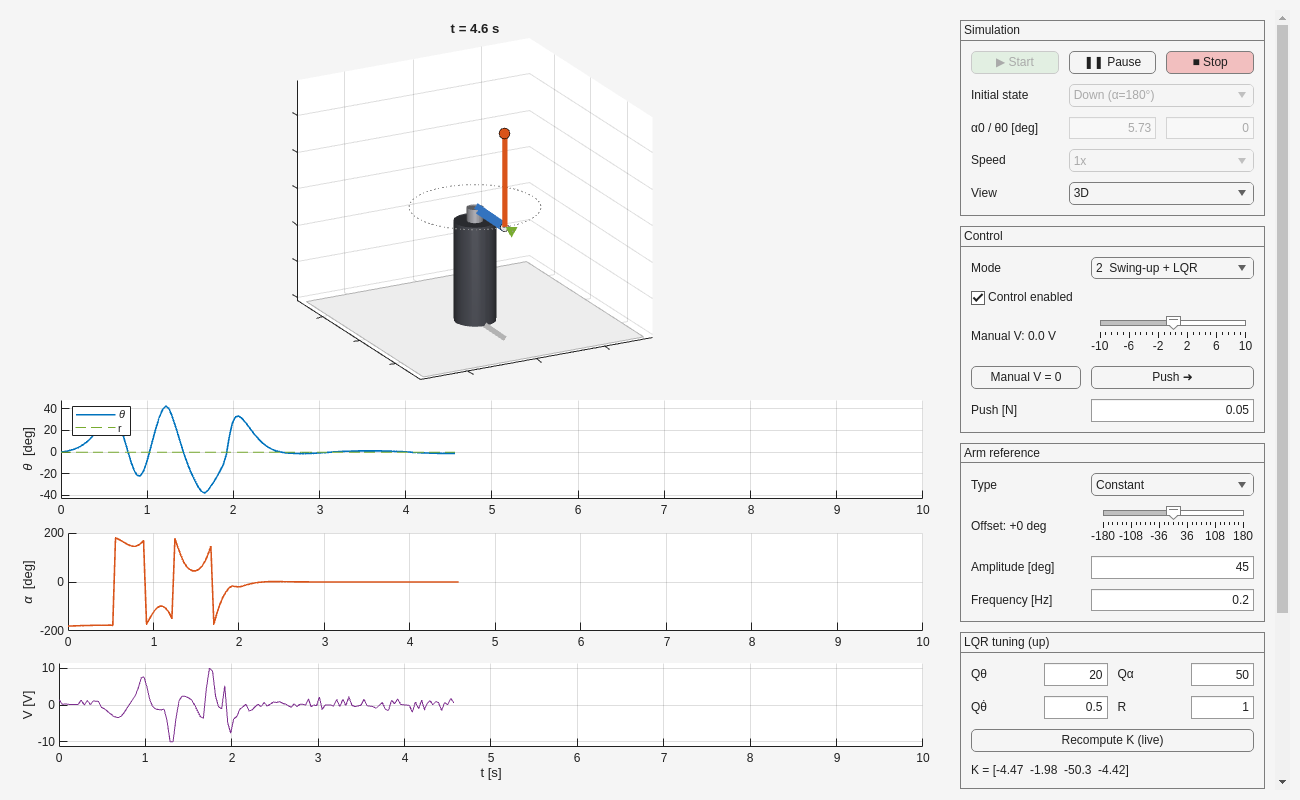
\includegraphics[width=\linewidth]{data/gui.png}
\caption{La GUI durante un swing-up en vivo, capturada a los \SI{4.5}{s}: el péndulo ya está equilibrado arriba.}
\label{fig:gui}
\end{figure}

\paragraph{La escena 3D.} La dibuja \code{rp\_draw} con primitivas gráficas de MATLAB: la base, el cuerpo del motor, el brazo (azul), el péndulo (naranja) y su sombra sobre la base. El círculo punteado es la trayectoria del extremo del brazo y el triángulo verde marca la referencia $r$. El punto de vista por defecto mira a lo largo del brazo en reposo, de modo que el balanceo del péndulo se ve de lado. Se puede girar con el ratón o elegir otro en la lista \textbf{View}:
\begin{itemize}
  \item \textbf{3D}: perspectiva por defecto (\code{view(62,20)}).
  \item \textbf{Top}: desde arriba; muestra directamente $\theta$.
  \item \textbf{Front} y \textbf{Side}: alzados a lo largo de $-y$ y de $+x$.
\end{itemize}
Las mismas vistas están disponibles desde código con \code{rp\_view(ax, nombre)}.

\paragraph{Uso típico.}
\begin{enumerate}
  \item Elegir el estado inicial (arriba con $\alpha_0$ y $\theta_0$ en grados, o abajo) y la velocidad de simulación.
  \item Pulsar \textbf{Start}. Desde ese momento, cualquier cambio de modo, referencia, tensión o pesos LQR se aplica en vivo.
  \item Con la ventana activa, las teclas $\leftarrow/\rightarrow$ aplican $\pm\SI{3}{V}$ mientras se mantienen pulsadas y la \textbf{barra espaciadora} da un empujón en la punta.
  \item Si aparece «SAFETY», hay que desmarcar y volver a marcar \emph{Control enabled}.
  \item \textbf{Stop} y después \textbf{Export last run}: los datos quedan en \code{rp\_res} y se representan con \code{rp\_plot\_results}.
\end{enumerate}

\begin{nota}
Para reproducir un ensayo por lotes con la animación, \code{rp.animate(res)} o \code{rp\_animate(res, P, 0.25)} (a un cuarto de velocidad, útil para ver el swing-up con calma).
\end{nota}
